
\begin{figure}[h]
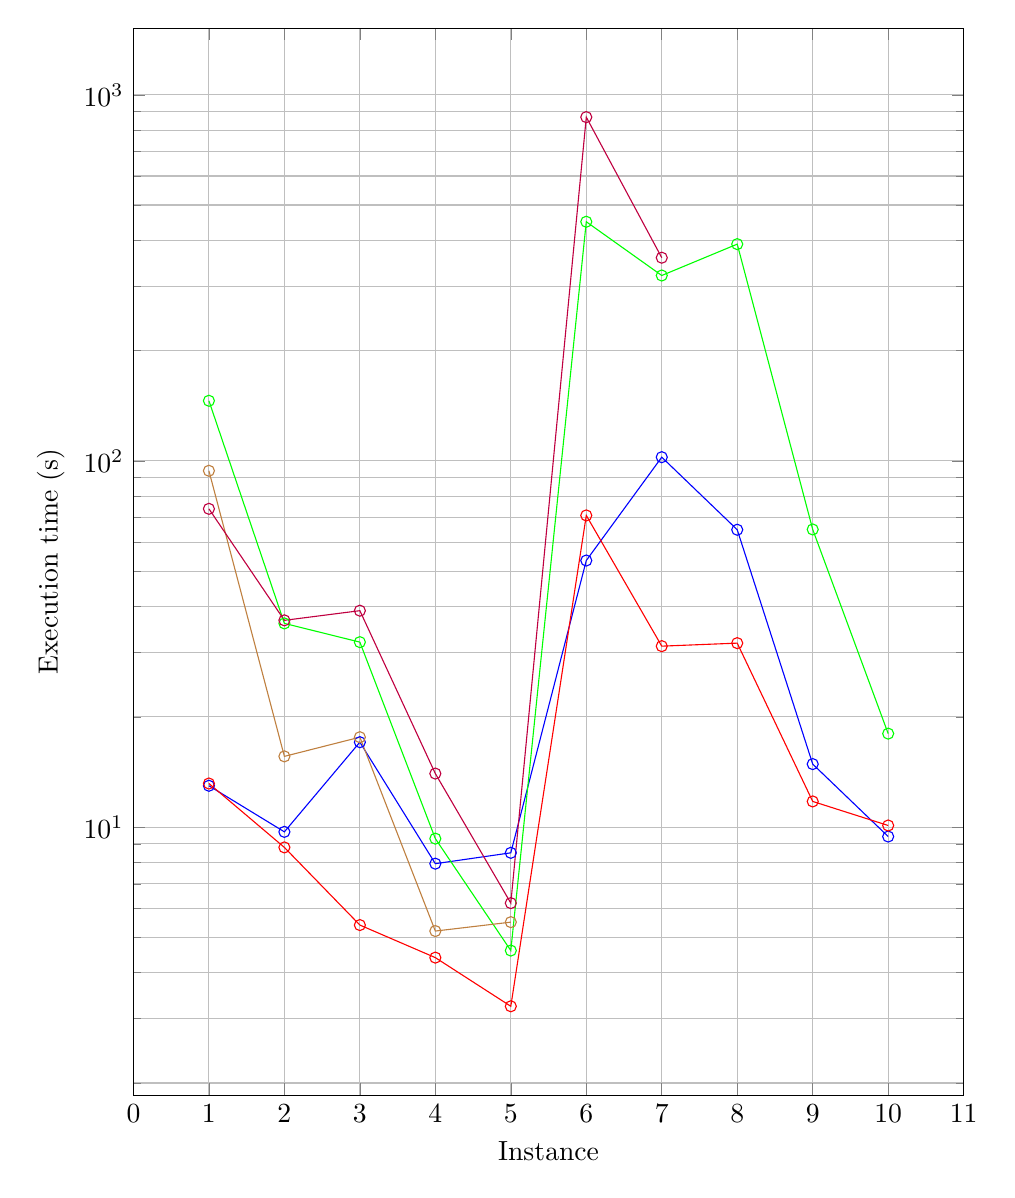
\begin{tikzpicture}
	\begin{axis}[width=\textwidth,height=100ex,
		xlabel=Instance,
		ylabel=Execution time (s), xmin=0, ymin=0, grid=both,
		ymode=log]
	
	
	% gurobi p3
\addplot[mark=o,color=blue] coordinates {
(1, 12.96708331)
(2, 9.704563172)
(3, 17.056811547)
(4, 7.944795782)
(5, 8.505190252)
(6, 53.456992427)
(7, 102.392618933)
(8, 64.881486922)
(9, 14.86064378)
(10, 9.421963416)
};

% gurobi p1
\addplot[mark=o,color=red] coordinates {
(1, 13.152454848)
(2, 8.8)
(3, 5.4)
(4, 4.4)
(5, 3.24)
(6, 70.99)
(7, 31.2)
(8, 31.8)
(9, 11.75)
(10, 10.1)
};

% cbc divisor 100
\addplot[mark=o,color=green] coordinates {
(1, 146)
(2, 36)
(3, 32)
(4, 9.3)
(5, 4.6)
(6, 450.1)
(7, 321)
(8, 391)
(9, 65)
(10, 18)
};

% cbc with random heuristic
\addplot[mark=o,color=brown] coordinates {
(1, 94)
(2, 15.6)
(3, 17.6)
(4, 5.2)
(5, 5.5)
};

% cbc with ff heuristic
\addplot[mark=o,color=cyan] coordinates {
};

% cbc with divisor 100
\addplot[mark=o,color=purple] coordinates {
(1, 74)
(2, 36.7)
(3, 39)
(4, 14)
(5, 6.2)
(6, 869)
(7, 359)
};

\end{axis}

\end{tikzpicture}%
\caption{Execution time for Gurobi on all instances with P1 (in red) and P3 (in blue) and for Cbc with P1, without any optimization (in green), using the random heuristic (in brown), using the farthest-first heuristic (in cyan) and using the VI attempt with divisor 100 (in purple). Cbc with P3 would take too much time and we would often not see the end of the computation, it is therefore not relevant to display it here along the others.}
\end{figure}
